\documentclass{article}
\usepackage{amsmath, amsthm, amsfonts, geometry, graphicx, blindtext}
\usepackage{natbib}
\usepackage[hidelinks,colorlinks=true,linkcolor=blue,citecolor=blue]{hyperref}
\usepackage{setspace}
\usepackage{indentfirst}
\usepackage{tabularx, booktabs, caption, float}
\usepackage{tikz, pgfplots}
\usepackage{multicol}
\usepackage{titlesec}
\usepackage{xcolor}
\pgfplotsset{compat=1.18, width=0.9\linewidth}

\captionsetup[table]{singlelinecheck=false, justification=raggedright, format=plain}

\setlength{\parindent}{1cm}
% \fontsize{8pt}{10pt}\selectfont
% \spacing{1.5}

\newgeometry{
    top = 0.75in,
    inner = 0.75in,
    outer = 0.75in,
    bottom = 0.75in
}

\renewcommand{\thesection}{\Roman{section}}
\titleformat{\section}
    {\fontsize{1em}{1.2em}\bfseries\centering\uppercase}{\thesection}{1em}{}

\renewcommand{\thesubsection}{\arabic{section}.\arabic{subsection}}
\titleformat{\subsection}
    {\fontsize{1em}{1.2em}\bfseries}{\thesubsection}{1em}{}

% \renewcommand{\thechapter}{\Roman{chapter}}

% For the chapter heading that has the title name after the line of the chapter number
% \titleformat{\chapter}[display]
    % {\fontsize{2em}{2.2em}\bfseries\centering}{\chaptertitlename\ \thechapter}{1em}{}
    % {\fontsize{2em}{2.2em}\bfseries\centering}{\thechapter}{0.25em}{}

% For the chapter heading that have the title name and chapter number in the same line
% \titleformat{\chapter}[hang]
%   {\fontsize{2em}{2.2em}\bfseries\centering\uppercase}
%   {\chaptertitlename\ \thechapter}{1em}{}


\title{{\Huge Lab Exercise 3}\\{\small CS ELEC 2C}}
\author{Alessandro Andrei Araza \and Joshua Kyle Entrata}
\date{\today}

\begin{document}

    \maketitle

    \begin{abstract}
        In this laboratory exercise, we developed a Convolutional Neural Network (CNN) model to classify hair types into three categories: Curly, Straight, and Wavy. The dataset presented some challenges, such as a limited number of samples. Our approach involved experimenting various preprocessing and model customization techniques. We constructed a multi-layer CNN and conducted several experiments to evaluate the impact of different preprocessing techniques, hyperparameter adjustments, and architectural configuration on model performance. Evaluation metrics, such as accuracy and loss plots, confusion matrices, and classification reports, were employed to measure the performance of our model. These experiments were strategically designed to achieve high accuracy and reduce overfitting. This exercise not only enhanced our understanding in CNNs for image classifcation but also challenged us to analyze and make decisions about creating an optimal model for practical applications.
    \end{abstract}

    \begin{multicols}{2}
        \raggedcolumns
        \section{Introduction}

\blindtext[3]

\subsection{Subtopic}

\blindtext

\subsection{Another Subtopic}

\blindtext[3]

        \section{Methodology}

The methodology of this lab exercise follows the usual process for machine learning problems/researches
\[
  \text{data} \to \text{preprocessing} \to \text{modeling} \to \text{evaluation}
\]

The preprocessing section mainly consists of splitting the dataset into training and testing data, checking the validity of data, as well as many others. The Convolutional Neural Network, like other neural networks, can be customized especially in the number of convolutional layers, different pooling methods, different kernels, etc. Unlike previous models, there really isn't much customization that could be done to them other than the hyperparameters to alter slightly how it works. But when it comes to CNNs, there's a lot more room for varying techniques. 

Later in experimentation, we will see how customizing the CNN can affect performance for detecting these hair types. For evaluation, the accuracy metric is used to measure the model's performance. 

\subsection{Data Acquisition and Preparation}

\subsubsection{Loading of Images}

A folder named 'hair_types' was manually imported in the repository containing 1000 images. Inside that folder has subdirectories for each hair type. Python Imaging Library (PIL) library was used to create a custom function of validating the images that was imported. It ensures that none of these images are corrupted and adhere to specific formats, such as PNG, JPG, and BMP. We exclude files that are not accepted by Tensorflow and does not match the specific formats, such as .WebP. After loading these images, 14 images were deleted and one image with a file type of .gif was also detected, but we didn't remove it because it is still valid for this experiment. This step is important to minimize potential issues during model training.

\subsubsection{Image Categorization}

This step involves segrating the images into three groups based on hair type labels found in their file paths. This will help in the structured training of the model by defining the classes of each images.

\subsubsection{Manual Inspection}

To ensure that no invalid images were overlooked, we manually inspected the images through file explorer. Through this inspection, it was detected that there is one image in 'Straight_Hair' subdirectory that is just a microphone logo. Thus, excluding this is beneficial to prevent the model learning unnecessary and wrong information.

\subsubsection{Image Display}

Using matplotlib, we displayed a sample from each category. This step is important to ensure the integrity and appropriateness of the labels and the image themselves.

\subsection{Preprocessing}

\subsubsection{Data Augmentation}

Initaially, we tried applying several data augmentation technicques, such as random horizontal and vertical flips, random rotations, and random zooms. However, we didn't apply data augmentation in the final model, which will be discussed on the Experiments section.

\subsubsection{Splitting Dataset}

To ensure generalizability of this model, we utilized Tensorflow's `image_dataset_from_directory` method to split the image data into training and validation datasets. 20 \% of the data was allocated for validation. Additionally, we resize all images to a uniform \(256 \times 256\) pixels for consistency and batch them in sizes of 64. Splitting the data this way helps prevent overfitting by ensuring that the model does not memorize the training data and allows us to fine-tune the model parameters based on the performance metrics gathered from validation set.

\subsubsection{Sobel Edge Detection}

A custom preprocessing function was created to detect Sobel edges in the images. This technique highlights the edges within each image. This technique will be applied for both training sets and validation sets to ensure consistency in how images are presented to the model.

We generated 9 samples from the dataset to display sobel edges applied images.

\begin{figure}[H]
  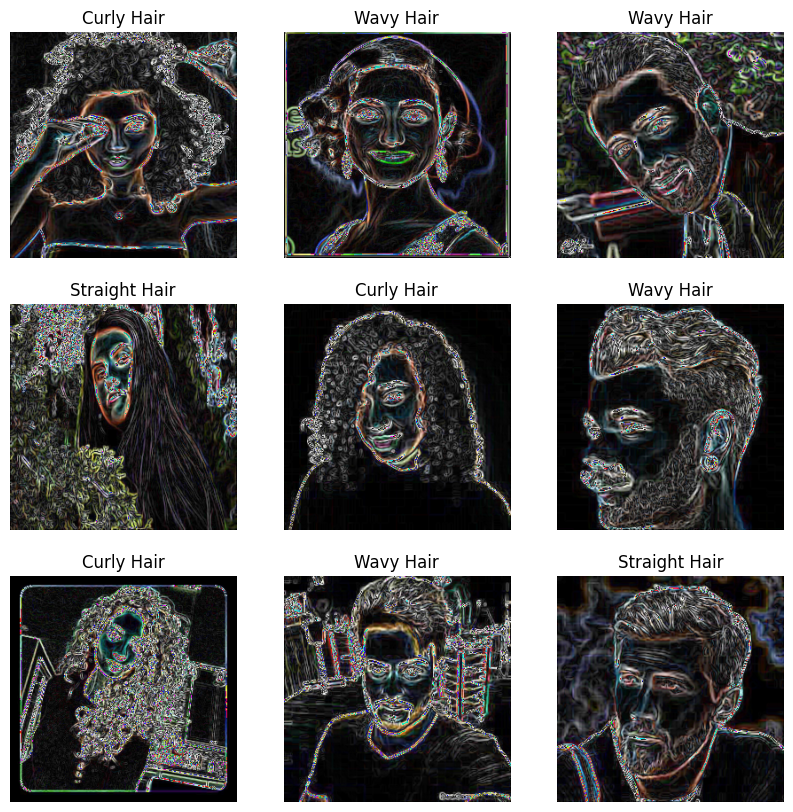
\includegraphics[width=\linewidth]{figures/sobel_edge_images.png}
  \caption{Hair Types Example with Sobel Edge}
  \label{fig:sobel_edge_hairtypes}
\end{figure}

\subsection{Modeling}

\subsubsection{Convolutional Neural Network Architecture}

In this step, we constructed a convolutional neural network (CNN) model using the Keras library's `Sequential` API. The network begins with a rescaling layer that normalizes the pixel values of the images from a range of 0 to 255 to a range of 0 to 1, enhancing the training efficiency. 

The architecture of our convolutional neural network (CNN) begins with the `Sequential` model framework from Keras, which allows layers to be added sequentially. 

1. Input Layer: This layer specifies the shape of the input data, which is 256x256, and adds three color channgels (RGB), making it \(256, 256, 3\).

2. Rescaling Layer: After the input layer, a `Rescaling` layer npormalizes the pixel values of the images from a range of 0 to 255 to a range of 0 to 1. This is important because it helps the model converge faster during the training stage.

3. First Convolution Layer: This layer uses 16 filters with a kernel size of 16 and a stride of 2. We also did not added padding in the input (`valid padding`). The dilation rate is set to 1, which keeps the kernel compact.

4. Activation Function: Every after convolution layer, a Rectified Linear Unit (ReLU) activation function is applied. This is used to introduce non-linearity to the model and solves the vanishing gradients issue.

5. Batch Normalization: This normalization technique is applied to help standardizing the data by normalizing the activation of the convolution layer.

6. Pooling Layer: After that, `MaxPooling2D` layer is applied to reduce the spatial dimentions of the output. It summarizes the features in a 2x2 window with the maximum value.

7. Dropout Layer: A dropout layer is introduced with a rate of 0.25 to help prevent overfitting by randomly setting a fraction of input unit to 0 during training.

8. Other Convolution Layers: The process above is repeated three more times with different filter and kernel sizes. The filters increase while the kernel size decrease as the process continue. For the last two convolution layers, max pooling and dropout were excluded.

9. Global Average Pooling: After the last convolutional layers, a `GlobalAveragePooling2D` layer is applied, which calculates the average value of each feature map and outputs a tensor that is smaller in size. This can help reduce the dimensionality of the feature maps and prevent overfitting. 

10. Flattening: After that, a `Flatten` layer then converts these features into a single vector. This helps maintain all the information from the feature maps and connect the convolutional layers to the fully connected layers.

10. Dense and Output Layers: The feature vector coming from the Flattening layer is fed into a dense layer of 32 neurons, followed by a dropout layer with a rate of 0.5, and then an activation function of ReLU. The final output layer will consists of 3 neurons (one for each hair type) with a `softmax` activation function.

\subsubsection{Training the Model}

The model was compiled with the Adam optimizer, using a learning rate of `1e-4` and categorical cross-entropy loss function because the dataset consist of multiple classes. The training was conducted over 50 epochs, using both training and validation datasets.

\begin{figure}[H]
  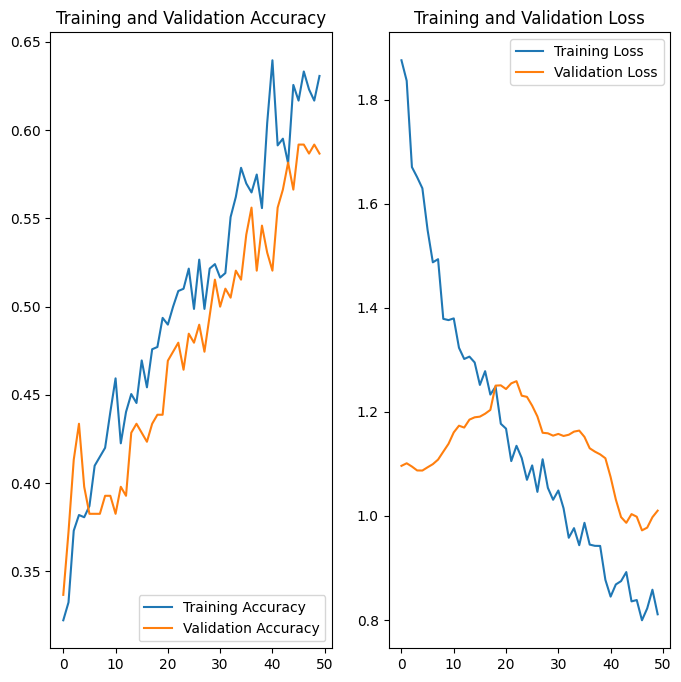
\includegraphics[width=\linewidth]{figures/training_validation_results.png}
  \caption{Training and Validation Results}
  \label{fig:results}
\end{figure}

\subsection{Evaluation}

To evaluate the performance of the convolutional neural network, we utilized different techniques that visually and quantitavely assess its effectiveness:

1. Accuracy and Loss Plots: We generated line plots to compare the training and valiation accuracy, as well as the training and validation loss over the epochs. These plots are important for us to understand the model's learning progress and see if it is overfitting or not.

2. Confusion Matrix: We created a confusion matrix from `sklearn.metrics` to visually inspect the performance of the model across different classes. It can also help us identify misclassifications in the model.

3. Classification Metrics Report: We utilized the `classification_report` from `sklearn.metrics` to see the results of the precision, recall, and F1-score for each class. 

4. Image Prediction: Finally, to demonstrate the effectiveness of the model in predicting the hair type of the image, we used the `predict` method to see the percentage of each classes based on a single image.
        \section{Experiments}

The objective of this experiment is to classify images into three hair types. To achieve this, we tested different hyperparameters, explored various preprocessing tecniques and experimented in creating the optimal CNN architecture. The primary goals in this experiment were to optimize evaluation metrics and minimize overfitting, ensuring robust model performance.

\subsection{Adjustment of Image Size and Batch Size}

The initial image size was set to \(64 \times 64\) pixels. While this smaller dimension allowed us to train the model faster, it compromised the quality of the training images, potentially eliminating important information for accurate classification. Conversely, increasing the image size to \(512 \times 512\) pixels significantly increased the training time to almost 30 minutes, which was impractical for our computational resources. Our experiments was conducted on a laptop with specifications of a GTX 1660Ti graphics card, a Ryzen 7 4800H processor, and 32GB of RAM.

Thambawita et al. (2021) \cite{smith2021edge} discussed in their paper that the performance of the classification model is dependent upon the resolution of images, but it is important to consider the trade-off between image size and the time needed for training the model. Considering these factors, we opted to use an image size of \(256 \times 256\) pixels. This resolution provides an optimal balance between image quality and manageable training times. 

\begin{figure}[H]
    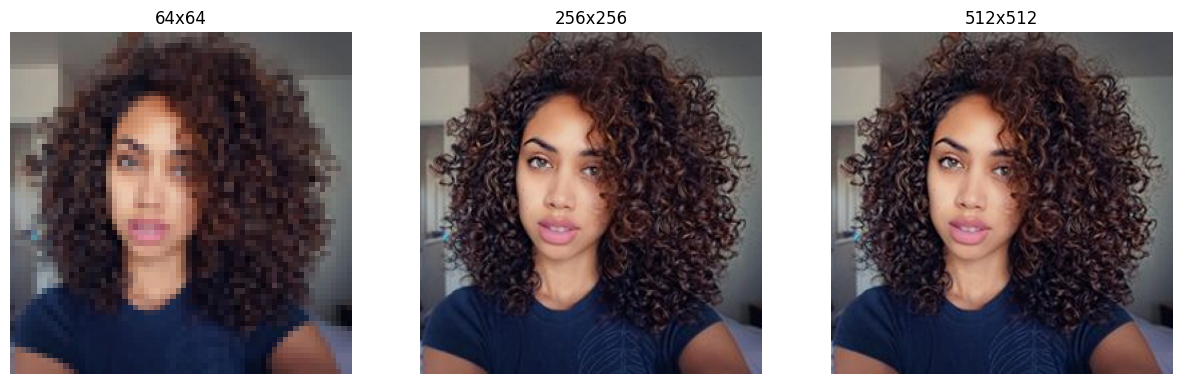
\includegraphics[width=\linewidth]{figures/image_sizes.png}
    \caption{Different Image Resolution}
    \label{fig:image_sizes}
  \end{figure}

Regarding the batch size, we experiments with sizes that are divisible by our image size, such as 32, 64, and 128. The batch size of 64 was chosen as it offers an efficient balance between minimizing the memory usage during training while providing a reliable estimate of the gradient. 

For the batch size, we used 64. We tested using batch size of 128 and 32 for this model since they are all divisible by 256 which is the image size, but we opted to continue using 64 for a better balance of requiring less memory in training and the accuracy of the estimate of the gradient.

\subsection{Preprocessing}

During the experimental phase, we utilized two preprocessing techniques in machine learning for image classification: Sobel Edge Detection and Data Augmentation. These methods were chosen based on their potential to improve model accuracy and minimize overfitting.

The models were evaluated under four different preprocessing scenarios to assess their impact:

\begin{itemize}
    \item No preprocessing
    \item With Sobel Edge Detection only
    \item With Data Augmentation only
    \item With both Sobel Edge Detection and Data Augmentation
\end{itemize}

\begin{table}[h]
\centering
\caption{Comparative Results of Different Preprocessing Techniques}
\label{tab:preprocessing_results}
\begin{tabular}{|l|c|c|p{5cm}|}
\hline
\textbf{Preprocessing Scenario} & \textbf{Training Accuracy} & \textbf{Validation Accuracy} & \textbf{Training Loss} & \textbf{Validation Loss} \\ \hline
No preprocessing & 0.6392 & 0.5431 & 0.7715 & 0.9983 \\ \hline
With Sobel Edge Detection only & 0.6145 & 0.5867 & 0.8398 & 1.0101 \\ \hline
With Data Augmentation only & 0.4311 & 0.5431  & 1.0880  & 0.9833 \\ \hline
With Sobel Edge Detection \& Augmentation & 0.4041 & 0.4112 & 1.1733 & 1.1114 \\ \hline
\end{tabular}
\end{table}

The results from each scenario are shown in the Table~\ref{tab:preprocessing_results}. Alongside these numerical results, we also provided plots of accuracy and loss to better illustrate the models' tendencies to overfit or underfit.

\begin{figure}[H]
  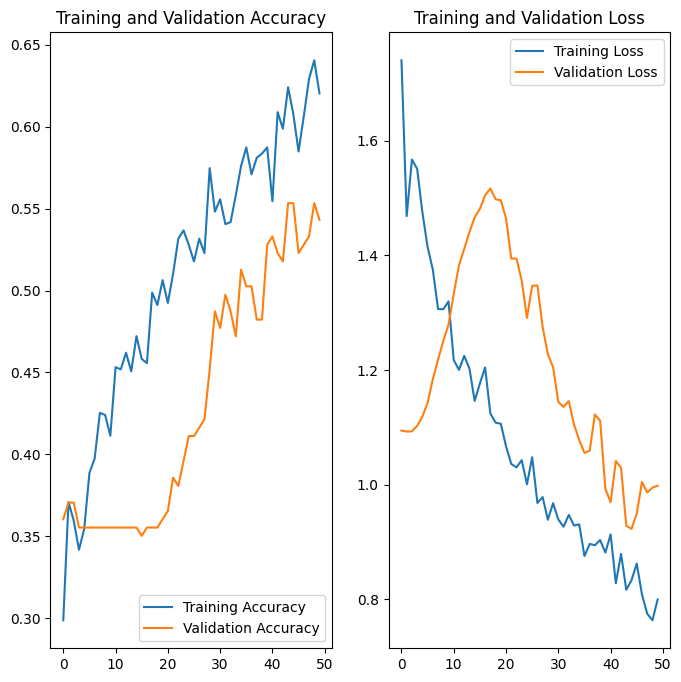
\includegraphics[width=\linewidth]{figures/without_preprocessing.png}
  \caption{No Preprocessing}
  \label{fig:no_preprocessing_plots}
\end{figure}

\begin{figure}[H]
  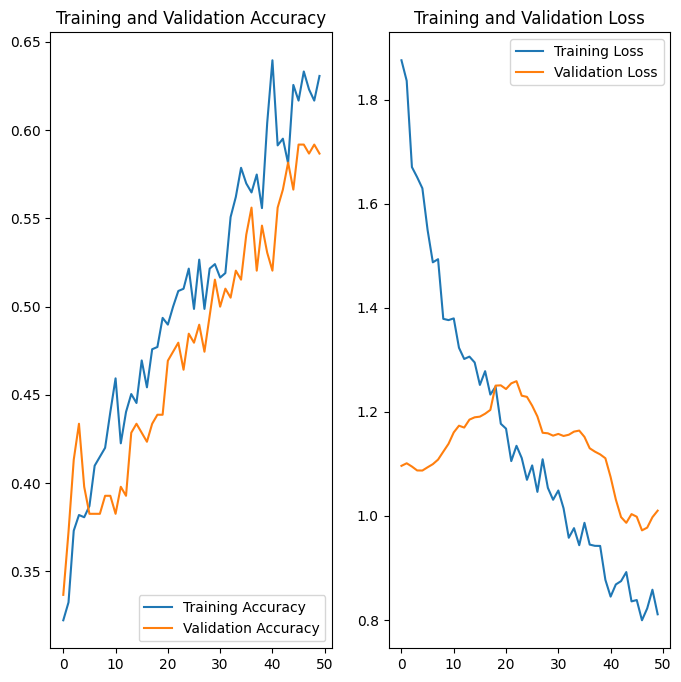
\includegraphics[width=\linewidth]{figures/training_validation_results.png}
  \caption{With Sobel Edge Detection only}
  \label{fig:sobel_edge_plots}
\end{figure}

\begin{figure}[H]
  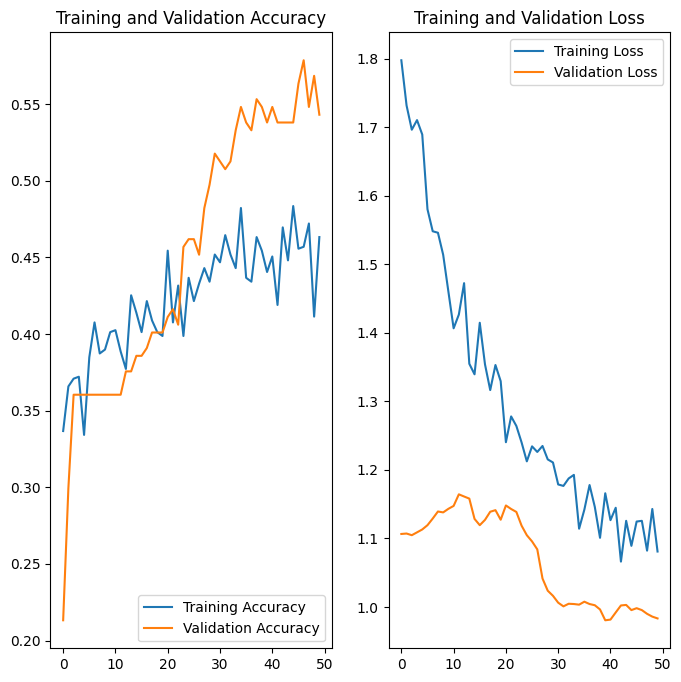
\includegraphics[width=\linewidth]{figures/with_data_aug.png}
  \caption{With Data Augmentation only}
  \label{fig:data_aug_plots}
\end{figure}

\begin{figure}[H]
  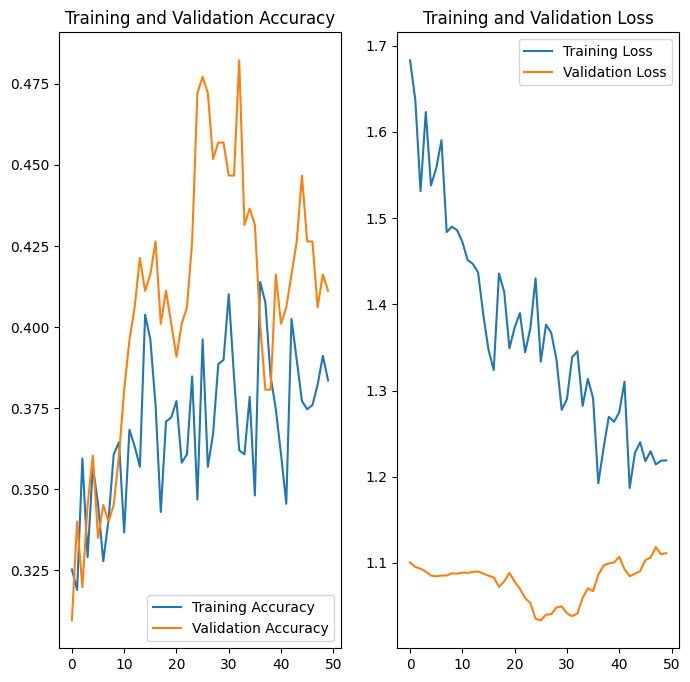
\includegraphics[width=\linewidth]{figures/with_data_aug_and_sobel_edge.png}
  \caption{With both Sobel Edge Detection and Data Augmentation}
  \label{fig:sobel_edge_and_data_aug_plots}
\end{figure}

The use of sobel edge detection help improved object detection and segmentation, notably improving hair boundary delineation in the images as seen in Figure~\ref{fig:sobel_edge_hairtypes}. Given our dataset only consists of 987 valid images, data augmentation was important in addressing the limited data situation. Despite its benefits, the best model performance was obseved with Sobel Edge Detection only, leading us to exlude data augmentation in next phases.

\subsection{Modeling}

\subsubsection{Convolutional Layers}


\subsubsection{Pooling Layers}

\subsubsection{Batch Normalization}

\subsubsection{Dropout Layers}

\subsubsection{GlobalAveragePooling2d and Flattening}

% discuss here the changing of hyperparameters in the cnn model


\subsubsection{Training the Model}

% discuss the experiments done in the compilation and training of datasets


        \section{Discussion}

\subsection{Sobel Edge Detection and Highlighting hair Edges}

Training a neural network can be a very tricky task; a lot of interconnecting parts can easily influence the other. The influence of one simple can be seen from the experimentation in each part of the process. For example, in previous lab exercises, adding or removing just one preprocessing technique can often be seen as futile or irrelevant. Oftentimes, in order to truly leverage preprocessing in the old machine learning models, these techniques need to be combined together. However there is a limit to how much preprocessing one should apply to the data, as introducing more interpolation, variance, or overall noise can be detrimental to the performance of the machine learning model.

Using Table \ref{tab:preprocessing_results} as an example, using Sobel Edge Detection (SED), it reduces overfitting when using the model without any preprocessing methods as the baseline for metrics. While Sobel Edge Detection lowered the training accuracy by around 0.02, overfitting reduced by increasing the accuracy for the validation set by 0.04. Looking at the baseline model, the difference or distance between the accuracy of training and validation sets is much larger than the model that applied SED. 

% TODO: add images of inputs

Sobel Edge Detection allows the CNN to easily capture the features better. Due to SED highlighting the edges in the images, the CNN takes advantage of this modification as it can better look at how the hair flows for each sample. Looking at Figure FIGURE, hairs are no exception to the SED, strands (especially those in the edge of the person's hair) are highlighted and emphasized in the image usually as a white color or something that is in complete contrast with the color assigned to non-edges. Kernels can find these more easily therefore train more easily ultimately leading to a better performance.

\subsection{Data Augmentation and Noise}



        \section{Conclusion}

\blindtext[3]

    \end{multicols}

    % Include in the bibliography all that was uncited
    \newpage
    \bibliographystyle{apalike2}
    \bibliography{citations, bib_a} % Put the file name only of the .bib files
    % https://zbib.org/59898e1965a74f2f9d57017519db0564

\end{document}
